\documentclass[12pt,letterpaper]{article}
\usepackage[left=16mm,right=16mm,top=20mm,bottom=17mm,headheight=14pt,headsep=5mm]{geometry}
\usepackage{tikz}
\usepackage{fancyhdr}
\usepackage[T1]{fontenc}
\usepackage{lmodern}
\pdfmapfile{+lm.map}
\renewcommand{\familydefault}{\sfdefault}
\setlength{\parindent}{0pt}
\pagestyle{fancy}
\fancyhf{}
\fancyhead[L]{\small Week 76 / Substitution strips / Letter tiles}
\fancyfoot[L]{\footnotesize Bellingham Math Circle / Week 76 / F76-M-v1}
\fancyfoot[R]{\footnotesize\thepage}
\renewcommand{\headrulewidth}{0pt}
\renewcommand{\footrulewidth}{0pt}
\begin{document}
Adults: print at 100\% (Actual size), on card stock if you have it, and cut along every line. One page makes 80 tiles, 20 mm square: 40 A and 40 B, enough for two kits of 36 (18 A and 18 B) with 8 spare. The B tiles are shaded so the two piles sort quickly; the letter is what counts. These tiles have not yet been tried with children.

\vspace{6mm}
\begin{center}
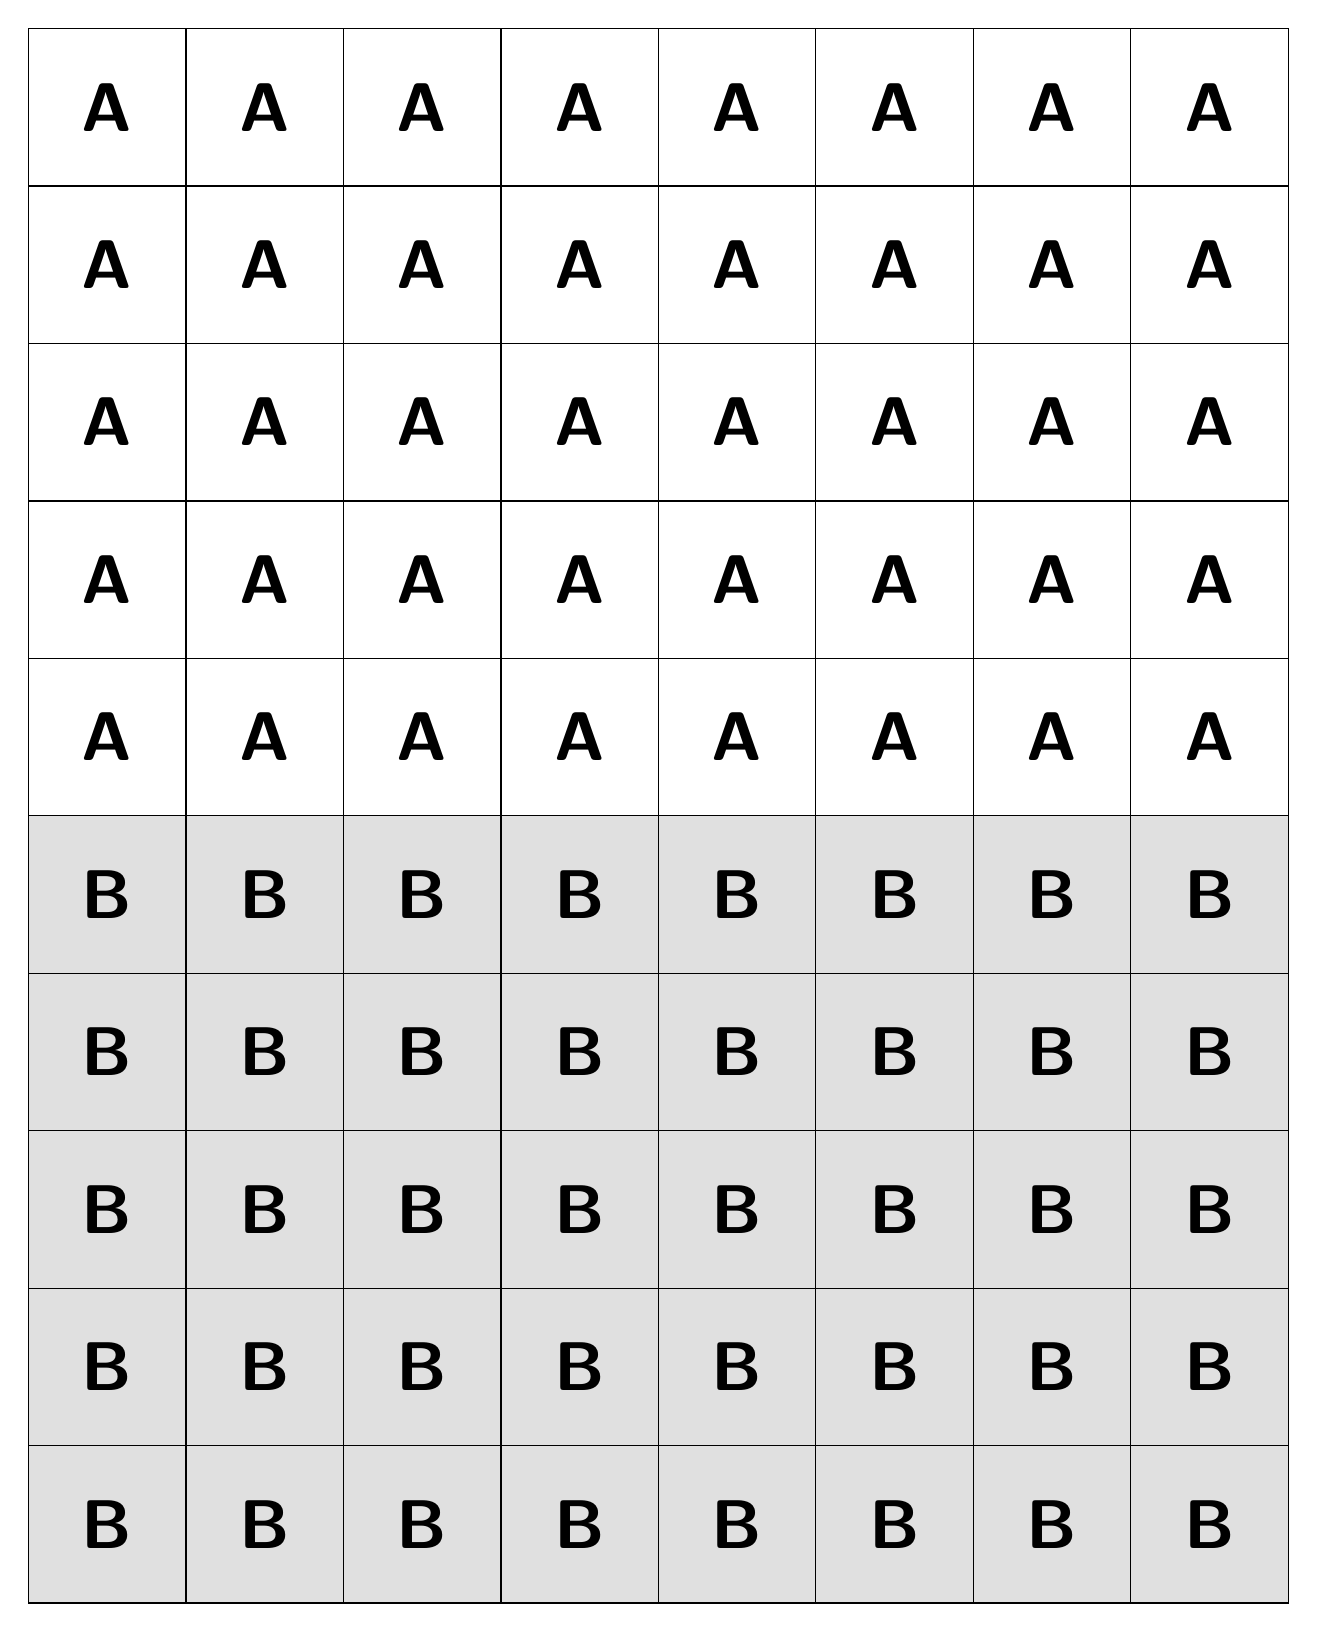
\begin{tikzpicture}[x=1mm,y=-1mm]
\foreach \r in {0,...,9} {
 \foreach \c in {0,...,7} {
  \ifnum\r<5
   \draw[line width=.5pt] (\c*20,\r*20) rectangle ++(20,20);
   \node[font=\fontsize{30}{30}\selectfont\bfseries] at (\c*20+10,\r*20+10) {A};
  \else
   \draw[line width=.5pt,fill=black!12] (\c*20,\r*20) rectangle ++(20,20);
   \node[font=\fontsize{30}{30}\selectfont\bfseries] at (\c*20+10,\r*20+10) {B};
  \fi
 }}
\end{tikzpicture}
\end{center}
\end{document}
